\documentclass[tikz,border=2pt]{standalone}
\usepackage{amsmath,amssymb}
\usepackage{tikz}
\usetikzlibrary{arrows.meta}

\begin{document}
% A binary integer program in two variables: only the four corners of the unit square are
% candidates; a constraint such as y_1 + y_2 <= 1 then removes (1,1).
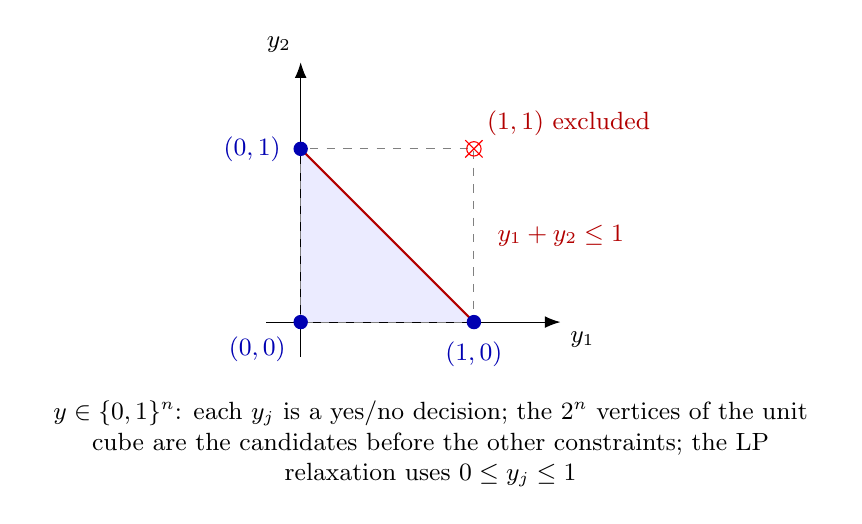
\begin{tikzpicture}[x=2.2cm, y=2.2cm, every node/.style={font=\small}, >={Latex[length=2mm]}]
	\fill[blue!8] (0,0) -- (1,0) -- (0,1) -- cycle;
	\draw[->] (-0.2,0) -- (1.5,0) node[below right] {$y_1$};
	\draw[->] (0,-0.2) -- (0,1.5) node[above left] {$y_2$};
	\draw[gray, dashed] (0,0) rectangle (1,1);
	\draw[red!70!black, thick] (1,0) -- (0,1);
	\node[red!70!black, font=\small, anchor=west] at (1.08,0.5) {$y_1+y_2\le1$};
	\foreach \p in {(0,0),(1,0),(0,1)} {\fill[blue!70!black] \p circle (2.6pt);}
	\node[blue!70!black, font=\small, anchor=north east] at (-0.03,-0.03) {$(0,0)$};
	\node[blue!70!black, font=\small, anchor=north] at (1,-0.06) {$(1,0)$};
	\node[blue!70!black, font=\small, anchor=east] at (-0.06,1) {$(0,1)$};
	\draw[red] (1,1) circle (2.6pt);
	\draw[red] (0.95,0.95) -- (1.05,1.05); \draw[red] (0.95,1.05) -- (1.05,0.95);
	\node[red!70!black, font=\small, anchor=south west] at (1.02,1.02) {$(1,1)$ excluded};
	\node[anchor=north, align=flush center, text width=10cm] at (0.75,-0.4) {$y\in\{0,1\}^n$: each $y_j$ is a yes/no decision; the $2^n$ vertices of the unit cube are the candidates before the other constraints; the LP relaxation uses $0\le y_j\le1$};
\end{tikzpicture}
\end{document}
